%ajouter draft pour voir débordement

%%%%%

\documentclass[12pt,french]{article}


\usepackage[utf8]{inputenc}
\usepackage[T1]{fontenc}
\usepackage{lmodern}
%règles mes marges et format papier
\usepackage{geometry} %modif marge et formet
\geometry{left=3cm,right=2cm,top=2.5cm,bottom=2.5cm}
\usepackage{amsmath, amssymb, amsthm}
\usepackage{fancyhdr} %pour les entêtes et bas de page
\usepackage{lastpage} %pour numéroter les pages charge la derniere page
\usepackage{graphicx} %pour inclure des img
\usepackage{dsfont}
\usepackage{float} %pour le placement des figures
\usepackage{hyperref} %pour mettre des liens hypertext
\usepackage{calc} %permet de calculer les marges pour encadrer les textes
\usepackage{color, xcolor} %gère les couleurs
\usepackage{babel}
\usepackage{listings} %pour afficher le code annexe
% Ajout du package glossaries 
\usepackage{glossaries} 
% Création du glossaire 
\makeglossaries

%pour afficher le code de manière esthétique
\lstset{
  aboveskip=3mm,
  belowskip=-2mm,
  backgroundcolor=\color{white},
  basicstyle=\footnotesize,
  breakatwhitespace=false,
  breaklines=true,
  captionpos=b,
  commentstyle=\color{red},
  deletekeywords={...},
  escapeinside={\%*}{*)},
  extendedchars=true,
  framexleftmargin=16pt,
  framextopmargin=3pt,
  framexbottommargin=6pt,
  frame=tb,
  keepspaces=true,
  keywordstyle=\color{blue},
  language=C,
  literate=
  {²}{{\textsuperscript{2}}}1 {⁴}{{\textsuperscript{4}}}1
  {⁶}{{\textsuperscript{6}}}1
  {⁸}{{\textsuperscript{8}}}1
  {€}{{\euro{}}}1 {é}{{\'e}}1 {è}{{\`{e}}}1 {ê}{{\^{e}}}1 {ë}{{\¨{e}}}1
  {É}{{\'{E}}}1 {Ê}{{\^{E}}}1 {û}{{\^{u}}}1 {ù}{{\`{u}}}1 {â}{{\^{a}}}1
  {à}{{\`{a}}}1 {á}{{\'{a}}}1 {ã}{{\~{a}}}1 {Á}{{\'{A}}}1 {Â}{{\^{A}}}1
  {Ã}{{\~{A}}}1 {ç}{{\c{c}}}1 {Ç}{{\c{C}}}1 {õ}{{\~{o}}}1 {ó}{{\'{o}}}1 
  {ô}{{\^{o}}}1 {Õ}{{\~{O}}}1 {Ó}{{\'{O}}}1 {Ô}{{\^{O}}}1 {î}{{\^{i}}}1
  {Î}{{\^{I}}}1 {í}{{\'{i}}}1 {Í}{{\~{Í}}}1,
  morekeywords={*,...},
  numbers=left,
  numbersep=10pt,
  numberstyle=\tiny\color{black},
  rulecolor=\color{black},
  showspaces=false,
  showstringspaces=false,
  showtabs=false,
  stepnumber=1,
  stringstyle=\color{gray},
  tabsize=4,
}

%Personalisation En tête
\pagestyle{fancy}
\renewcommand\headrulewidth{1pt}
%\setlength{\headheight}{2.5cm}

\fancyhead[L]{Projet de 60 heures}
\fancyhead[C]{
\includegraphics[scale=0.22]{header.png}}
\fancyhead[R]{2022 - 2023}


\renewcommand\footrulewidth{1pt}
\fancyfoot[L]{BALLEJOS Lilian}
\fancyfoot[C]{\thepage/\pageref{LastPage}}
\fancyfoot[R]{CHARPIN Etienne}
%Fin personalisation En Tête

%table des matieres
\renewcommand\thesection{\Roman{section}}
\renewcommand\thesubsection{\arabic{subsection}}
\renewcommand\thesubsubsection{\thesubsection.\arabic{subsubsection}}


\begin{document}

\newgeometry{margin=2.5cm}
\begin{titlepage} %page d'acceuil

  
  \begin{center}
  	
\includegraphics[scale=0.35]{isima.png}
  \end{center}
  
  %\hspace*{\stretch{1}}%espace horizontal entre les 2 images
  %
\includegraphics[scale=0.25]{deco.png}
  
  \vspace*{3cm} %espace de 2.5cm en dessous des images
  
  \hrule
  
  \begin{center}
  	\large
  	Rapport d'élève ingénieur
  	
  	Projet de 2ème année
  	
  	Filière: Génie Logiciel et Systèmes Informatiques
  	
  	\huge
  	\textbf{Projet Fullstack de Révision de Parole}
  \end{center}

\hrule
  
  \vspace*{1.8cm} 
  
  \begin{center}
 
  	
  \Large Présenté par : \textbf{BALLEJOS Lilian et CHARPIN Etienne}
  
   \end{center}

\vspace*{7cm}
  
  
  
  
  	\begin{minipage}{.45\linewidth}
  		\begin{flushleft}
  			\textbf{Responsable ISIMA: YON Loic}
  			
  			\textbf{Soutenance : Jeudi 23 Mars}
  		\end{flushleft}
  	\end{minipage}
  	\hfill
  	\begin{minipage}{.45\linewidth}
  		\begin{flushright}
  			\textbf{Projet de 60 heures}
  			
  			\textbf{Année Scolaire 2022 - 2023}
  		\end{flushright} 
  	\end{minipage}
  	
  	\vspace*{2cm} 
  	
    Campus des Cézeaux. 1 rue de la Chebarde. TSA 60125. 63178 Aubière CEDEX
    	

\end{titlepage}

\restoregeometry



\normalsize\tableofcontents %place la table des matières

\newpage

\section{Contexte du projet}

\subsection{Introduction au Full Stack}

Pour commencer l'explication du projet, nous allons faire une brève introduction au \textbf{Full Stack}.

\medskip

Lors d'un projet informatique de Développement Web, l'architecture du logiciel va être séparé en plusieurs parties distinctes: la partie côté serveur dit le "back" puis la partie côté utilisateur dite le "front".

\medskip

La partie front va être chargé sur le moteur de recherche de l'utilisateur et donc le code sera disponible et exploitable par n'importe quel utilisateur du site web (par exemple le code HTML ainsi que le code Javascript).

\medskip

A l'inverse la partie back va géré tous les comportements communs que l'on doit garder côté serveur (interagir avec la base de donnée, contacter une API ....).

\medskip

Lorsqu'on parle de Full Stack, on parle donc du développement de ces deux aspects. D'où le terme Full Stack qui peut se comprendre comme "travailler tout les aspects du projet".

\medskip

Dans ce projet nous allons vous montrer comment nous avons implémenter un projet Full Stack avec un back en NodeJs à l'aide du module "Express" et un front à l'aide du framework Angular. 

\begin{figure}[H]
	\centering
	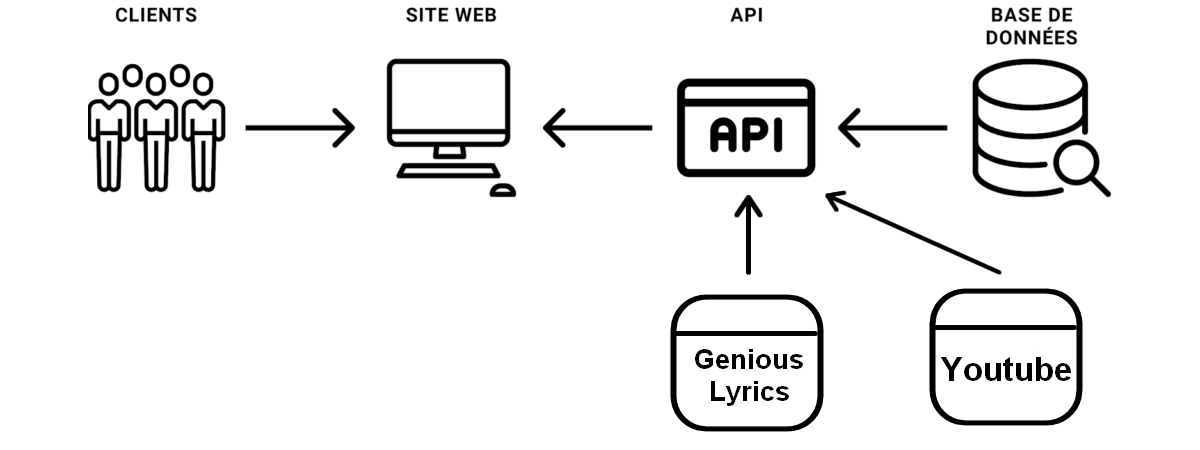
\includegraphics[scale=0.4]{fullstack.png}
	\caption{Organigramme de notre Application Fullstack}    
\end{figure}

\section{Réalisation et conception}

\subsection{Nos choix}

\subsubsection{Le Back de notre site}

Pour la partie back de notre projet nous avons choisit de prendre NodeJs avec le module "Express".

\medskip

L'un de nous avait déjà travaillé sur cette technologie donc cela permettait pour l'un, de ne pas partir de zéro et d'améliorer ses connaissances et pour l'autre de découvrir une nouvelle technologie possiblement très utile pour notre filière de développement à l'ISIMA.

\medskip

De plus, NodeJs est une technologie plus récente que d'autres langages qui peuvent gérer le côté serveur (comme PHP par exemple). Ainsi le module Express que nous utilisons est toujours maintenu à jour.

\medskip

Avec Express, nous pouvons en quelques minutes implémenter une API assez facilement et parfaitement fonctionnelle. Cela nous a permit de bien scinder la partie front et back de notre projet.
Nous pouvons par exemple citer l'exemple de PHP où la partie serveur et client est parfois mélanger dans les mêmes fichier.

Ici, nous avons le back dans un dossier et le front dans autre et ces deux aspects sont parfaitement indépendant ! On peut par exemple lancer le back pour faire des tests dessus sans toucher au front.

La partie front va pouvoir communiquer avec la partie front à l'aide de requête envoyé à celui-ci auquel il va répondre.

\bigskip

Au niveau de l'organisation de notre back, nous avons séparé celui-ci en différentes couches.

\medskip

\begin{itemize}
	\item \textbf{Couche "Controller"}: réceptionne les requêtes et appelles les fonctions nécessaires en fonction de la demande. Répond ensuite aux requêtes. Elle correspond au fichier \textit{listen.js}
	\item \textbf{Couche "Business"}: effectue tous les calculs de notre API, on implémente dans celle-ci toutes les fonctions nécessaires au bon fonctionnement de l'API (communication avec d'autres API, création de trou à compléter dans les paroles etc...). Elle correspond à tous les fichiers \textit{gestion\_*.js} sauf "\textit{gestion\_database.js}"
	\item \textbf{Couche "Base de donnée"}: effectue toutes les requêtes à la base de donnée et renvoie les données récupérées. Elle est appelées par la couche business. Elle correspond au fichier \textit{gestion\_database.js}.
	
\end{itemize}

\bigskip

\begin{figure}[H]
	\centering
	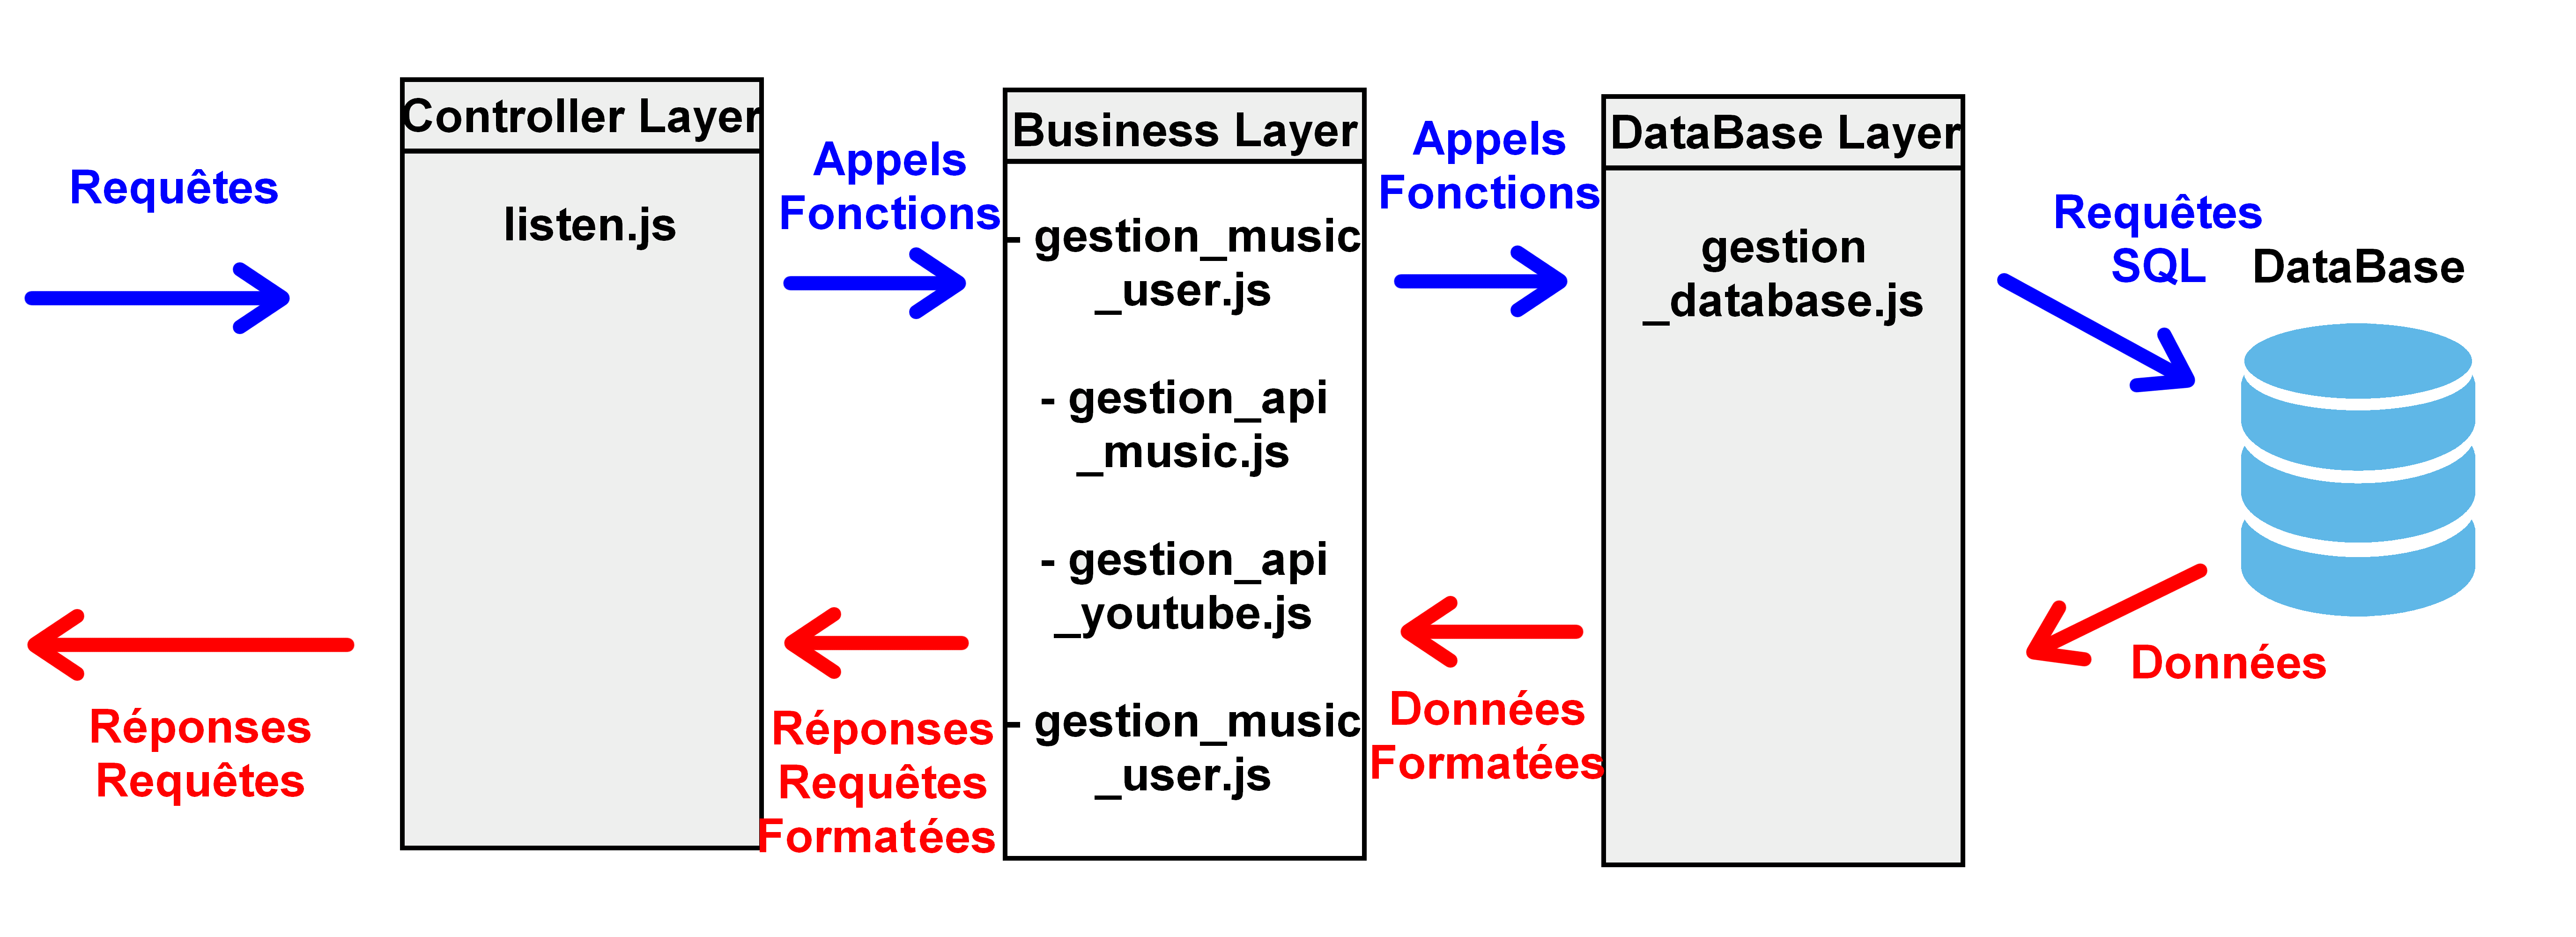
\includegraphics[scale=0.1]{api_couche.png}
	\caption{
	L'organisation de l'API}    
\end{figure}

\bigskip

Pour démarrer notre API, on lance le fichier \textbf{server.js} qui place notre API sur le port voulu de notre machine
Ensuite, il se connecte à la base de donnée. Enfin, après que tout cela soit fait, on active les différents contrôleur de l'API et on est prêt à recevoir des requêtes !

\begin{figure}[H]
	\centering
	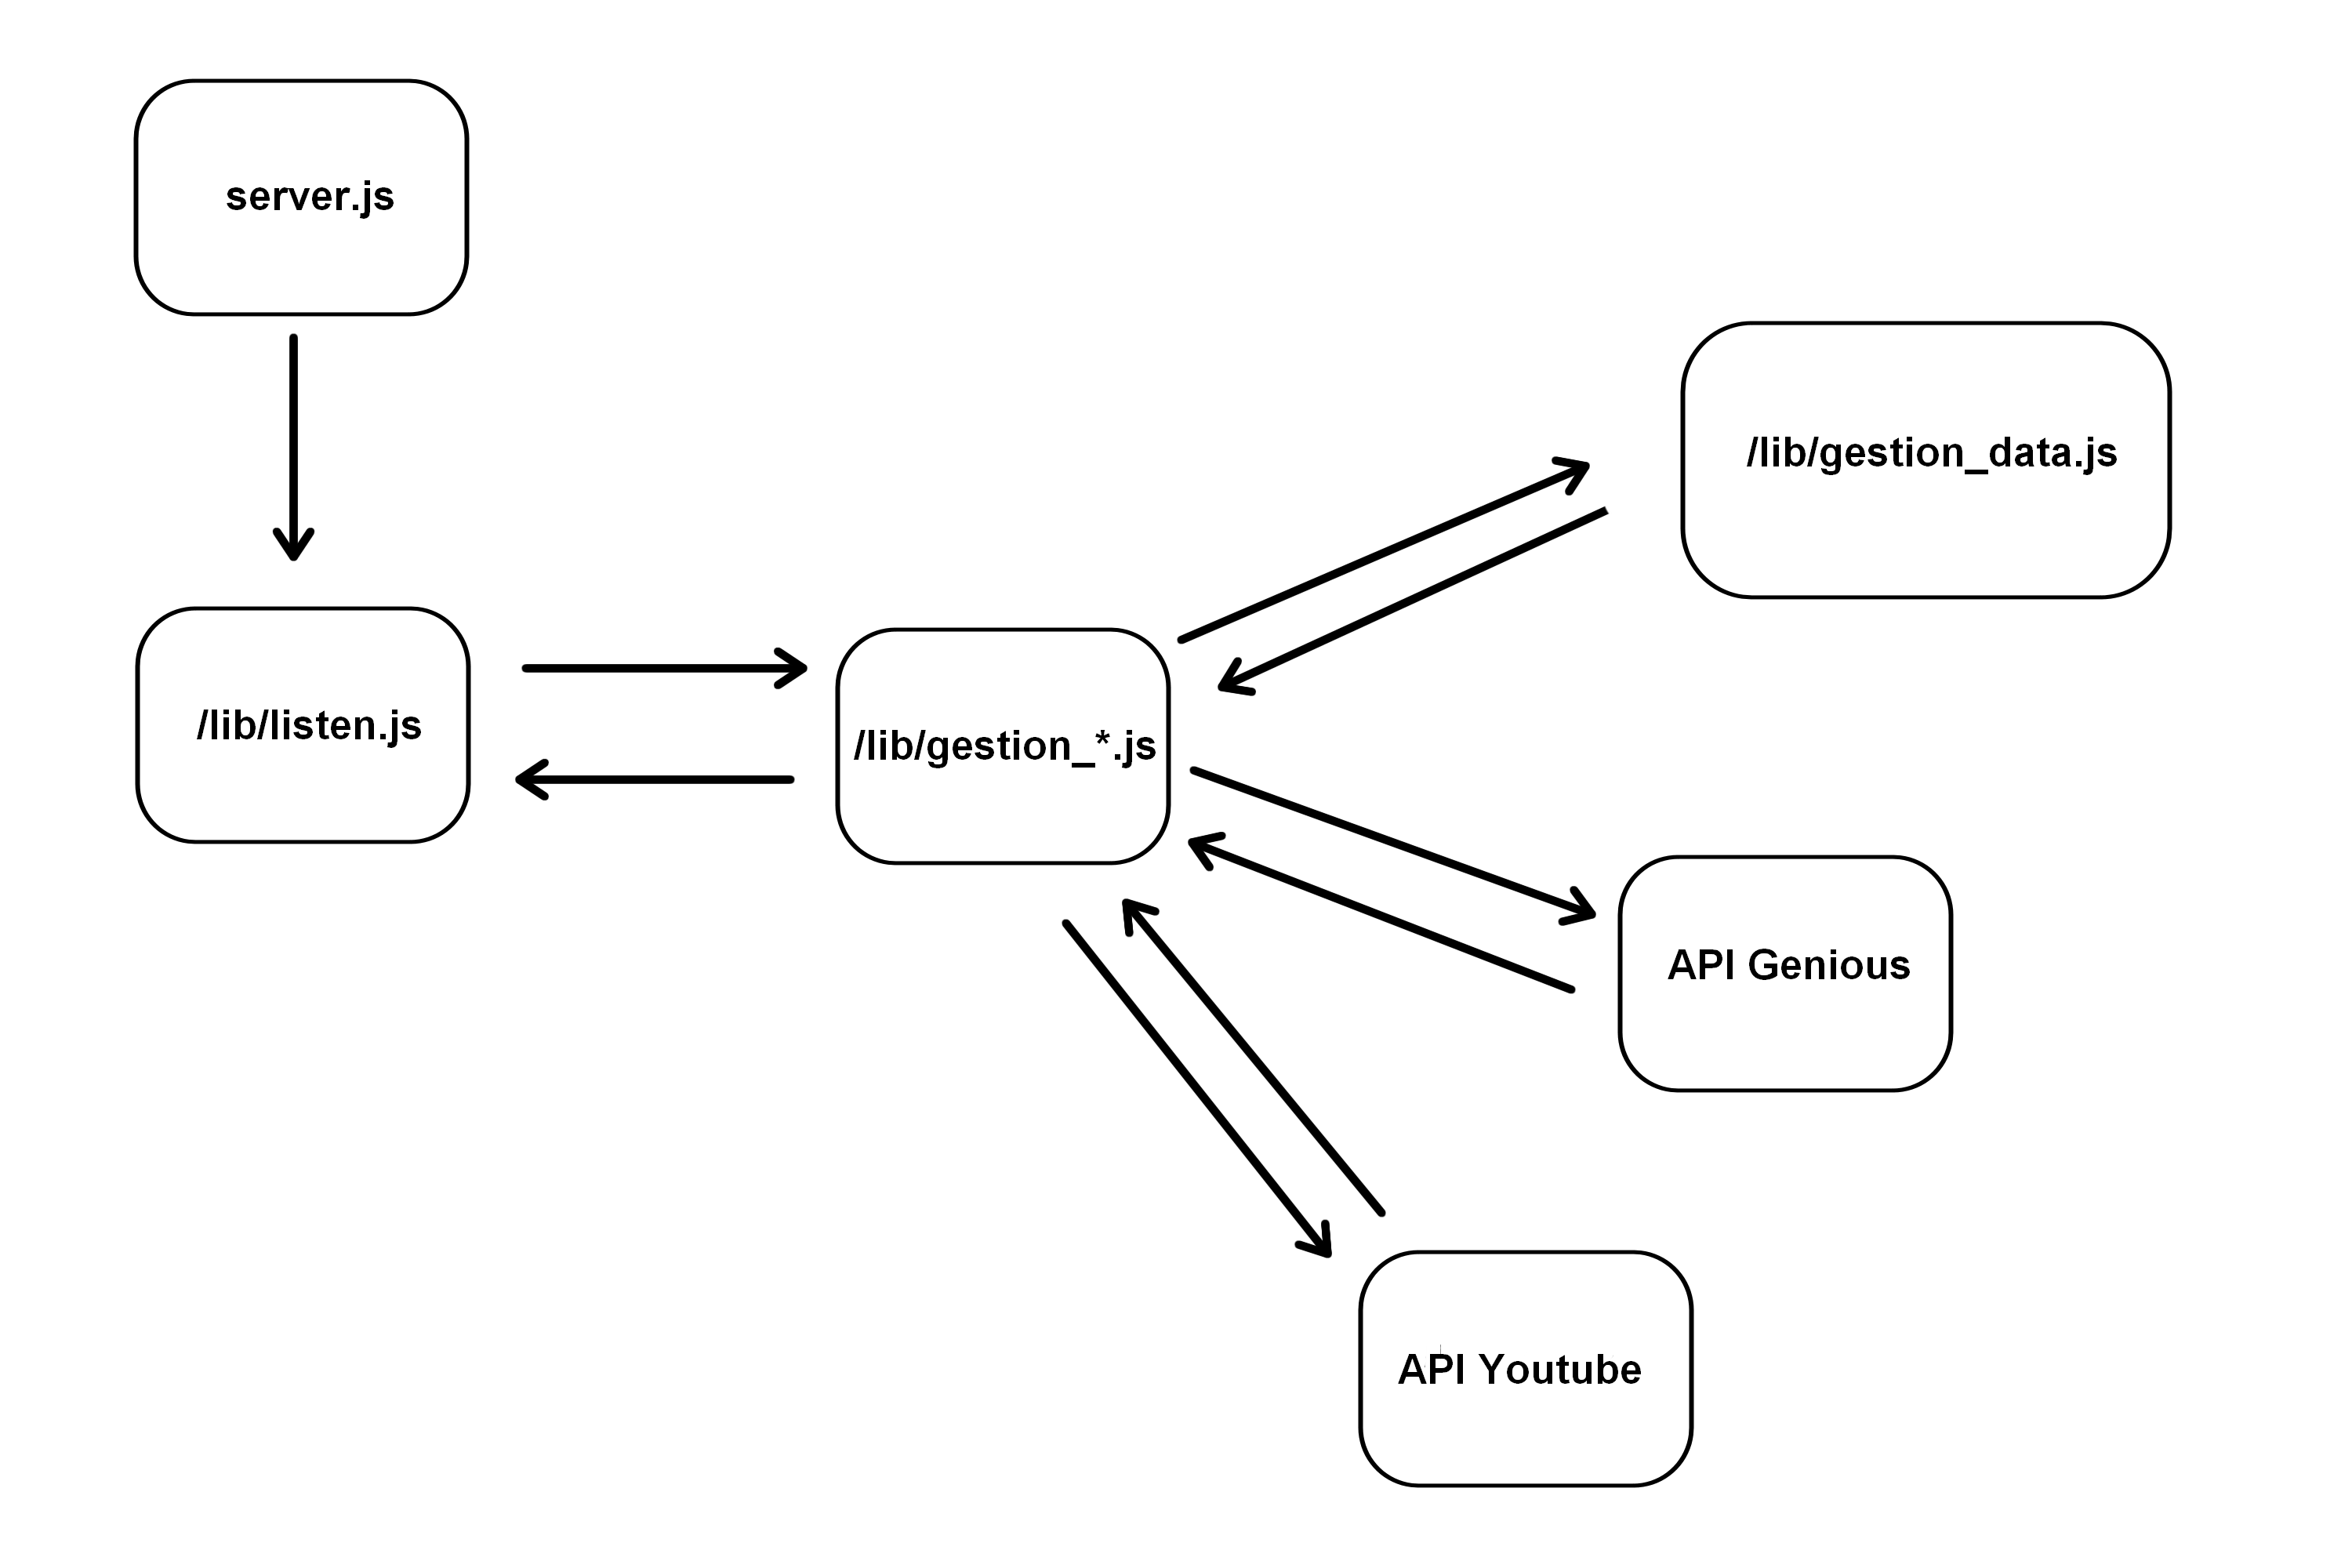
\includegraphics[scale=0.16]{api.png}
	\caption{Architecture de l'API}    
\end{figure}

\medskip

On peut voir ici que l'on communique avec d'autres APIs publiques ! On vous explique cela plus en détail après.

\subsubsection{Le Front}

Pour la partie Front nous avons prit le choix de prendre un Framework car ces technologies sont plus évolués pour effectuer des comportements complexes.

\medskip

L'un des gros avantages de ces technologies est de pouvoir séparer notre application en plusieurs composants que l'on va pouvoir faire interagir les un avec les autres ou encore inclure les un dans les autres !

Cela permet de structurer plus proprement et efficacement une application.

\medskip

De plus les Framework sont des outils très puissant avec de nombreuses fonctionnalités pré-implémentées Cela nous permet de ne pas avoir besoin de réinventer la roue est de nous concentrer sur nos implémentations personnelles.

\medskip

Ainsi nous avons hésité entre le Framework Angular et ReactJS qui sont les plus courants et les plus utilisés de nos jours.

Notre choix c'est finalement porté sur Angular car nous étions familiarisés avec ce Framework suite à des projets personnelles.
Le deuxième avantage de ce Framework est que sur la version que nous utilisons, il est nativement utilisé avec Typescript qui permet de faire des applications plus clair en typant les variables et objets utilisés.
De plus, chaque composant généré est composé d'un fichier HTML, un fichier SCSS et un fichier Typescript ce qui permet de bien scinder les 3 différents aspects importants du front qui sont respectivement dans l'ordre le corps d'une page, son style et son comportement.

\bigskip

En plus d'Angular, nous avons utilisé le framework \textbf{Bootstrap} pour avoir des éléments graphiques classes et au goût du jour. Par exemple, notre barre de navigation a été stylisé grâce à ce framework.

De plus, nous avons utilisé \textbf{PrimeNg} qui est une bibliothèque de composants Angular. Nous y retrouvons dedans plein d'éléments déjà créés très pratique comme des dossiers (que nous avons utilisé pour la partie utilisateur) ou encore des boutons déjà stylisés.


\subsubsection{Choix des APIs}

Nous avons dû utilisé pour ce projet deux APIs publiques de deux entreprises différentes.

\medskip

Ces APIs nous permettent de récupérer des informations comme par exemple des paroles de musique et nous ont été très utiles. Pour chacune d'elle nous avons dû nous inscrire sur le site de la documentation afin d'obtenir un token pour communiquer avec elles.

\paragraph{Gestion des lecteurs vidéos avec paroles de musique \\\\} 

La première est l'API de \textbf{Youtube} de l'entreprise \textbf{Google}. Nous lui demandons via une requête le meilleur résultat pour une recherche avec les mots clefs "\textit{nom musique}" + "\textit{nom artiste}" + "lyrics".

L'API nous répond en envoyant une liste des 5 vidéos sur sa plateforme qui corresponde le mieux à la recherche et nous, nous renvoyons le résultat numéro 1 à la partie utilisateur afin d'afficher le bon URL dans le lecteur.

\paragraph{Récupération des paroles de musique \\\\}

Notre second objectif était de trouver une API qui pourrait nous fournir les paroles de musique et qui couvre donc un très grand nombre de celle-ci.

\medskip

Nous nous sommes tout d'abord penché sur l'API \textbf{ChartLyrics} puis nous nous sommes rendu compte que celle-ci était trop incomplète. L'API étant américaine nous avions dessus très peu de musique française ce qui est très dommage au vu de notre projet.

\medskip

Ainsi, nous nous sommes ensuite penché sur une autre API d'un site très connu qui couvre de très nombreuses musiques très diversifiées: \textbf{Genious Lyrics}.

Le problème de cette API est que dû à des problèmes de droit sur les paroles de musique (gérés en France par la \textbf{SACEM}), nous ne pouvons pas obtenir les paroles de musique directement via des requêtes.

La solution est la suivante: l'API nous fournit le lien vers la page web du site \textbf{GeniousLyrics}. Nous récupérons ce lien et grâce à du Web scraping nous arrivons a récupérer les paroles.

Dans l'ordre la méthode pour récupérer les paroles d'une musique est donc la suivante: 

\medskip

\begin{itemize}
	\item On contacte l'API Genious Lyrics et on lui demande l'url de la page du site qui contient les paroles
	\item On aspire ensuite tout le code HTML de la page web du site
	\item Les paroles étant toujours dans la même balise HTML, on les récupère tout en ignorant le reste du contenu de la page
	\item Enfin on formate les paroles pour qu'elle soit plus adapter à de l'apprentissage.
\end{itemize}

\medskip

\subsection{Le déroulement du projet}

Notre façon de travailler était comparable à une méthode agile de développement.

C'est à dire que nous avons séparé le projet en différentes parties comme vous l'avez vu plus tôt (partie parole, partie user ...)

A chaque partie du projet, nous avons effectué un sprint durant lequel on suivait toujours le même schéma de travail:

\medskip

\begin{itemize}
	\item On implémente ou modifie la base de donnée
	\item On relie la partie serveur (back) du projet avec la base de donnée.
	\item On implémente les fonctionnalités nécessaires côté serveur
	\item On relie la partie user (front) à la partie serveur (back)
	\item On teste la fonctionnalité implémentée
\end{itemize}

\begin{figure}[H]
	\centering
	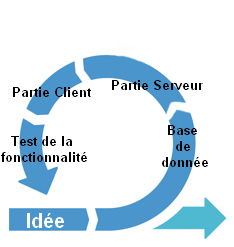
\includegraphics[scale=1]{agile.png}
	\caption{Les différentes étapes d'ajout d'une fonctionnalité}    
\end{figure}

\medskip

Au final, on a effectué à la toutes fin un embellissement de la partie utilisateur (front) car il est très important d'avoir une interface utilisateur très agréable d'utilisation pour faciliter l'interaction avec notre application.

\medskip

Voyons maintenant en précisions ce qu'impliquait chaque partie d'un sprint de notre projet.

\subsubsection{Exemple complet d'un Sprint}

\paragraph{Modification de la base de donnée \\\\}

A chaque nouveau sprint on regardait tout d'abord si une modification de la base de donnée était nécessaire.

\medskip

Si c'est le cas, on reconstruisait notre base de donnée en rajoutant les nouvelles tables et colonnes nécessaires.

Cela implique de modifier le script \textbf{setupDatabase.js} pour que nous ayons chacun de notre côté, en local, exactement la même base de donnée.

Lorsque cela était fait, on effectuait chacun de notre côté des tests en local sur nos machines afin de vérifier que nos bases de données avait le même comportement.

\paragraph{Mise en lien de la base de donnée avec notre partie serveur \\\\}

Ensuite, on reliait la base de donnée à la partie serveur.

\medskip

Le principe est le suivant: on créait des requêtes SQL qui permettent de récupérer les données dont on a besoin pour les futurs implémentations.

On inclut ensuite ces requêtes dans le code Javascript de notre back dans le fichier \textit{gestion\_database.js}

Enfin on crée dans la "couche business" toutes les fonctions nécessaires pour formater les données comme il nous faut.

C'est durant cette partie aussi que l'on a créé les fonctions qui envoie des requêtes HTTP à des APIs si nécessaire. Comme avec la base donnée, après avoir reçu les données on les formate afin de mieux les exploiter dans le front. 

\paragraph{Mise en lien de la partie serveur avec la partie utilisateur\\\\}

Au final, il ne nous restait plus qu'à créer côté client les nouveaux composants Angular nécessaires pour implémenter la nouvelle fonctionnalité. Ensuite, on avait juste à créer les requêtes à envoyer à notre partie serveur pour récupérer les éléments nécessaires côté client.



\subsubsection{Nos différents Sprints effectués}

Nous avons effectué ainsi 3 sprints durant le développement de notre application web.

\begin{itemize}
	\item Le développement de la partie entrainement avec les paroles
	\item Le développement de la partie inscription/connexion 
	\item Le développement de la partie partie stockage des musiques avec les dossiers utilisateurs 
\end{itemize}


\subsubsection{Embellissement du front}

Au départ, nous avons cherché à développer une application fonctionnelle sans nous pencher de trop sur l'apparence. Nous avons essayé de développer toutes les fonctionnalités que nous voulions ajouter en nous assurant que celle-ci n'avait aucun bug.

\medskip

Après s'être assuré que tous fonctionné comme nous le souhaitions, nous avons décidé à la toute fin d'embellir le front. Nous avons pour cela utilisé nos connaissances en CSS ainsi qu'en Bootstrap.

\medskip

Ayant quelques notions d'IHM (interface homme machine), nous savons que l'apparence d'un site web est une étape primordiale du développement logiciel. En effet il ne faut pas par exemple utiliser des contrastes de couleur qui pourrait gêner certaines personnes comme les daltoniens.

De plus chaque éléments du site doit être intuitif et c'est ainsi que nous avons essayé de faire des fonctionnalités très simple d'utilisation (bouton simple, pas trop de détails ...).

\begin{figure}[H]
	\centering
	\begin{minipage}{.5\textwidth}
		\centering
		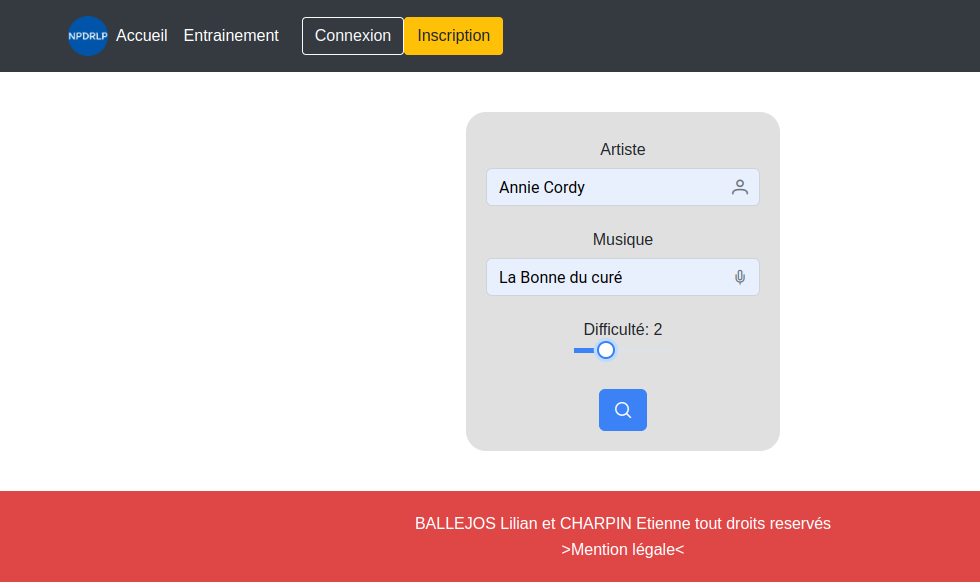
\includegraphics[scale=0.25]{avantfront.png}
	\end{minipage}%
	\begin{minipage}{.5\textwidth}
		\centering
		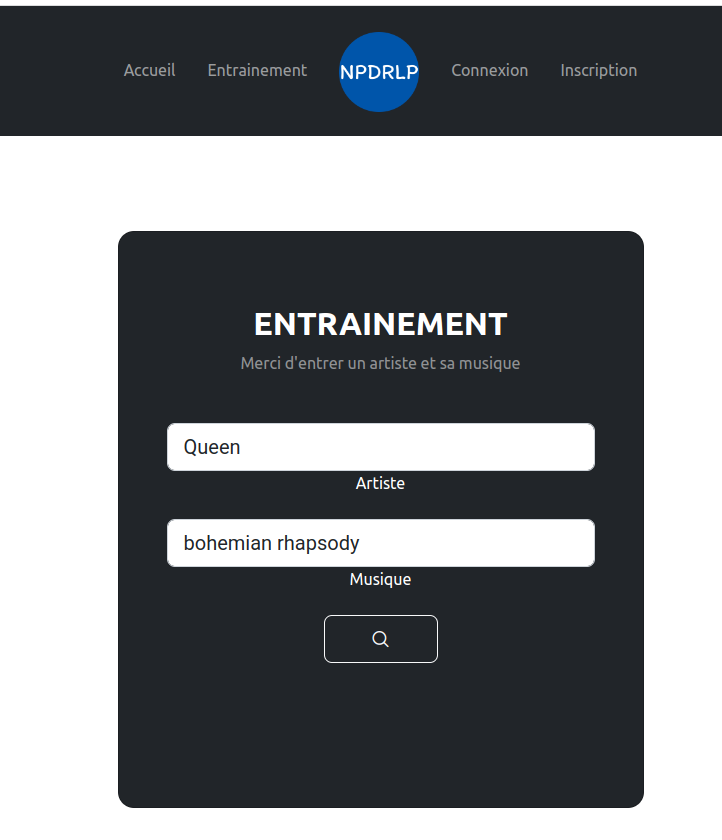
\includegraphics[scale=0.25]{apresfront.png}
	\end{minipage}
	\caption{Avant / Après de l'apparence de la partie client}    
\end{figure}

\section{Résultats et discussions}

\subsection{Prise en Main de l'Application Web}

\subsubsection{Arrivé sur le site}

Lors de votre arrivée sur le site, vous arrivez sur une page d'accueil défilante qui vous informe du concept de notre application , de qui nous sommes et de nombreuses autres informations.

Nous pouvons si nous le souhaitons changer le code source du site web afin de rajouter des éléments à l'accueil et cela sans difficulté !

\medskip

En haut, vous pouvez voir les différentes fonctionnalités de notre site web qui sont proposés dans le header.

On a donc la possibilité d'aller à l'accueil 
(là où nous sommes actuellement) mais aussi dans la partie entrainement. Nous pouvons aussi au choix nous inscrire où si cela est déjà fait de nous connecter !

Le header va changer en fonction de si vous êtes connecté ou non. Si vous êtes connecté, au lieu de la possibilité de s'inscrire ou se connecter, vous aurez la possibilité d'aller à votre menu utilisateur ou de vous déconnecter.

\textbf{IMAGE ACCUEIL}

\subsubsection{Partie Entrainement}

En arrivant dans la partie entrainement, un formulaire vous demande de renseigner à la fois une nom d'artiste ainsi que la musique que vous souhaitez apprendre.

\medskip

Si vous renseignez quelques choses de faux ou erroné, l'application affichera un message d'erreur vous informant que les paroles n'ont pas pu être trouvé.

\medskip

Si les informations renseignées sont justes, alors l'entièreté des paroles de la musique est affichée sur votre écran. En dessous de celle-ci vous trouverez un lecteur Youtube avec une vidéo de la musique recherchée.

\medskip

Enfin nous trouvons au dessus des paroles un bouton "Options" sur lequel nous pouvons cliquer.

Lors du clique sur celui-ci, un menu apparait sur la gauche avec deux fonctionnalités:

\begin{itemize}
	\item Sauvegarder la musique dans un dossier
	\item Changer la difficulté
\end{itemize}

\paragraph{Sauvegarder la musique dans un dossier \\\\}

Lorsque vous cliquez sur le bouton sauvegarder la musique, deux possibilités s'offre à vous. Si vous n'êtes pas connecté, nous allons vous informer qu'il faut que vous vous connectiez si vous souhaitez sauvegarder une musique. Sinon, une liste déroulante de tous vos dossiers apparait, il suffit de cliquer sur le dossier dans lequel vous voulez sauvegarder la musique pour lancer la phase de sauvegarde.

Après ce clique, une pop-up apparait vous demander de confirmer votre choix. Lorsque cela est fait une notification apparait en haut à droite de votre écran vous informant que la sauvegarde a été effectuée !

\paragraph{Changer la difficulté\\\\}

Un curseur vertical vous permet de changer la difficulté. Selon la difficulté choisit allant de 1 à 4, un certain nombre de trou vont apparaitre dans les paroles de la musique et le but de l'utilisateur est de les compléter. Un bouton "Valider" apparait aussi en bas des paroles afin d'effectuer une correction de vos réponses. Si la réponse est juste, la case se colorie en vert et vous ne pouvez plus modifier votre réponse, si elle est rouge c'est que c'est faux.

Vous pouvez voir au dessus des paroles un avancement du nombre de réponse juste par rapport au nombre de réponse attendu.

A noter que les trous sont disposés aléatoirement, si jamais vous modifiez la difficulté un nouveau pattern de trou sera appliqué aléatoirement.

\subsubsection{Inscription}

Lors de votre arrivé sur 






\end{document}
